%  LaTeX support: latex@mdpi.com
%  For support, please attach all files needed for compiling as well as the log file, and specify your operating system, LaTeX version, and LaTeX editor.

%=================================================================
\documentclass[remotesensing,article,submit,pdftex,moreauthors]{Definitions/mdpi}

%=================================================================
% MDPI internal commands - do not modify
\firstpage{1}
\makeatletter
\setcounter{page}{\@firstpage}
\makeatother
\pubvolume{1}
\issuenum{1}
\articlenumber{0}
\pubyear{2024}
\copyrightyear{2024}
%\externaleditor{Academic Editor: Firstname Lastname}
\datereceived{ }
\daterevised{ } % Comment out if no revised date
\dateaccepted{ }
\datepublished{ }
%\datecorrected{} % For corrected papers: "Corrected: XXX" date in the original paper.
%\dateretracted{} % For corrected papers: "Retracted: XXX" date in the original paper.
\hreflink{https://doi.org/} % If needed use \linebreak
%\doinum{}
%\pdfoutput=1 % Uncommented for upload to arXiv.org
%\CorrStatement{yes}  % For updates


%=================================================================
% Add packages and commands here. The following packages are loaded in our class file: fontenc, inputenc, calc, indentfirst, fancyhdr, graphicx, epstopdf, lastpage, ifthen, float, amsmath, amssymb, lineno, setspace, enumitem, mathpazo, booktabs, titlesec, etoolbox, tabto, xcolor, colortbl, soul, multirow, microtype, tikz, totcount, changepage, attrib, upgreek, array, tabularx, pbox, ragged2e, tocloft, marginnote, marginfix, enotez, amsthm, natbib, hyperref, cleveref, scrextend, url, geometry, newfloat, caption, draftwatermark, seqsplit
% cleveref: load \crefname definitions after \begin{document}

%=================================================================
% Please use the following mathematics environments: Theorem, Lemma, Corollary, Proposition, Characterization, Property, Problem, Example, ExamplesandDefinitions, Hypothesis, Remark, Definition, Notation, Assumption
%% For proofs, please use the proof environment (the amsthm package is loaded by the MDPI class).

%=================================================================
% Full title of the paper (Capitalized)
% \Title{Robot Team III: Scotty Strikes Back}
\Title{Visualization and Unsupervised Classification of Water Composition with UAV-based Hyperspectral Imaging and Generative Topographic Mapping}

% MDPI internal command: Title for citation in the left column
\TitleCitation{Title}

% Author Orchid ID: enter ID or remove command
\newcommand{\orcidauthorA}{0000-0002-5910-0183} % John
\newcommand{\orcidauthorB}{0000-0003-2688-648X} % Lakitha
\newcommand{\orcidauthorC}{0000-0002-9841-6703} % Shawhin
\newcommand{\orcidauthorD}{0000-0003-2657-3416} % Prabuddha
\newcommand{\orcidauthorE}{0000-0003-4265-9543} % David
\newcommand{\orcidauthorF}{0000-0003-0667-2345} % Ash
\newcommand{\orcidauthorG}{0000-0002-0126-218X} % Adam
% \newcommand{\orcidauthorH}{} % Gokul

% Authors, for the paper (add full first names)
\Author{John Waczak \orcidA{}, Adam Aker \orcidG{}, Lakitha O. H. Wijeratne \orcidB{}, Shawhin Talebi \orcidC{}, Ashen Fernando \orcidF{}, Prabuddha M. H. Dewage \orcidD{}, Mazhar Iqbal, Matthew Lary, David Schaefer, Gokul Balagopal, and David J. Lary *\orcidE{}}

%\longauthorlist{yes}

% MDPI internal command: Authors, for metadata in PDF
\AuthorNames{John Waczak, Adam Aker, Lakitha O. H. Wijeratne, Shawhin Talebi, Bharana Fernando, Prabuddha Hathurusinghe, Mazhar Iqbal, Matthew Lary, David Schaefer, Gokul Balagopal, and David J. Lary}

% MDPI internal command: Authors, for citation in the left column
 \AuthorCitation{Waczak, J.; Aker, A.; Wijeratne, L.O.H.; Talebi, S.; Fernando, B.; Hathurusinghe, P.; Iqbal, M.; Lary, M.; Schaefer, Balagopal, G.; D.; Lary, D.J.}
% If this is a Chicago style journal: Lastname, Firstname, Firstname Lastname, and Firstname Lastname.

% Affiliations / Addresses (Add [1] after \address if there is only one affiliation.)
\address[1]{%
Hanson Center for Space Sciences, University of Texas at Dallas, Richardson, TX 75080, USA;  john.waczak@utdallas.edu (J.W.); adam.aker@utdallas.edu (A.A.); lhw150030@utdallas.edu (L.O.H.W.); shawhintalebi@gmail.com (S.T.); ashen.fernando@utdallas.edu  (B.F.); pxh180012@utdallas.edu (P.M.H.D.); mazhar.iqbal@utdallas.edu (M.I.); MDL210001@utdallas.edu (M.L.); captdaveschaefer@gmail.com (D.S.); gokul.balagopal@utdallas.edu (G.B.);}

% Contact information of the corresponding author
\corres{Correspondence: david.lary@utdallas.edu} %; Tel.: (optional; include country code; if there are multiple corresponding authors, add author initials) +xx-xxxx-xxx-xxxx (F.L.)}


% Abstract (Do not insert blank lines, i.e. \\) 
\abstract{
Unmanned Aerial Vehicles (UAVs) equipped with hyperspectral imagers have emerged as an essential technology for the characterization of inland water bodies. The high spectral and spatial resolutions of these systems enable the retrieval of a plethora of optically-active water quality parameters via band ratio algorithms and machine learning methods. However, fitting and validating these models requires access to sufficient quantities of in situ reference data which are time-consuming and expensive to obtain. In this study, we demonstrate how the Generative Topographic Mapping (GTM), a Bayesian realisation of the Self Organizing Map (SOM), enables highly-detailed unsupervised classification and nonlinear endmember extraction of UAV acquired hyperspectral imagery. Specifically, the topographic relationship between classes maintained by the GTM presents an attractive alternative to other unsupervised approaches which do not provide a notion of similarity between learned classes. Using data collected across a North Texas pond, we apply the GTM to create a detailed map segmenting the area into distinct regions of interest. Further, by interpreting the learned classes as distinct endmembers, the GTM can be used to rapidly identify and map unique water constituents. We demonstrate this capability by using the GTM to map algal abundance as well as the dispersion of a rhodamine dye tracer released into the water.
}

% Keywords
\keyword{Hyperspectral Imaging; Remote Sensing; Unsupervised Classification; Endmember Extraction, Spectral Unmixing} 


%%%%%%%%%%%%%%%%%%%%%%%%%%%%%%%%%%%%%%%%%%
\begin{document}

%%%%%%%%%%%%%%%%%%%%%%%%%%%%%%%%%%%%%%%%%%
\section{Introduction}

Inland water bodies present a unique challenge to characterization by remote sensing imagery due to their complex spectral characteristics and small scale spatial variability. The broad bands of multi-spectral imagers coupled with the irregular shape of lakes and rivers results in pixels with highly mixed signals that are easily dominated by reflectance from shore and near-shore vegetation sources \cite{koponen2002lake, ritchie2003remote}. Recently, the combination of hyperspectral imaging with unmanned aerial vehicles (UAV) such as drones has emerged as a powerful approach to simultaneously address the spectral, spatial, and temporal limitations of traditional high-altitude and satellite-based collection \cite{adao2017hyperspectral,arroyo2019implementation}. UAV are significantly less expensive to deploy than their remote sensing counterparts, and low altitude flights enable centimeter-scale sampling while limiting the need for complicated atmospheric corrections \cite{banerjee2020uav}. However, the significant increase in data volume generated by these systems presents a new challenge, namely, how to efficiently extract water quality parameters of interest from intricate pixel spectra.

Significant research efforts have focused on the development of techniques and algorithms to retrieve water quality parameters from UAV-captured hyperspectral images (HSI). On-board compute installed alongside hyperspectral imagers can enable the rapid evaluation of spectral indices from HSI band ratios \cite{horstrand2019uav}. These band ratios and polynomial combinations of bands have been used to successfully invert optically-active water quality parameters such as turbidity directly from UAV acquired imagery \cite{vogt2016near, zhang2022selection}. Supervised machine learning techniques such as tree-based models, support vector machines, and neural networks have also been used to estimate a plethora of parameters such as colored dissolved organic matter, chlorophyll a, blue-green algae, and suspended sediment concentrations \cite{keller2018hyperspectral, lu2021retrieval}. The calibration and evaluation of these data-driven models demand a significant volume of coincident, in situ data. This can be addressed by coordinating UAV flights with reference data collection using autonomous robotic boats \cite{robot-team-1, robot-team-2}. Nevertheless, this approach relies on prior knowledge of expected sources in order to select appropriate reference instruments for model validation. The presence of unanticipated contaminants cannot be directly identified in this sensing paradigm. 

Extending the capabilities of UAV-based hyperspectral imaging to enable water quality monitoring in real-time scenarios where contaminant sources may not be known in advance requires two additional capabilities: dimensionality reduction techniques to permit the visual comparison of HSI, and endmember extraction techniques which can identify spectral signatures corresponding to unique sources within the imaging scene. In remote sensing where reference data are typically sparse, many approaches have been explored. For example, principal component analysis (PCA) and t-distributed stochastic neighbor embedding (tSNE) are dimensionality reduction methods commonly used to reduce HSI to two or three dimensions for visualization \cite{tyo2003principal,zhang2015hyperspectral}. Similarly for endmember extraction there are a variety of established approaches including geometric methods like vertex component analysis, statistical methods like k-nearest neighbors and non-negative matrix factorization (NMF), and deep learning methods based on autoencoder architectures \cite{heylen2014review,nascimento2005vertex, Feng2022HyperspectralUB, cariou2015unsupervised, su2019daen, borsoi2019deep, palsson2020convolutional}. Methods based on linear mappings like PCA and NMF are often too restrictive for HSI where the assumption of linear mixing is easily broken. However, the increased complexity of nonlinear methods like tSNE and autoencoders often lead to significant increases in computation time. An ideal approach should enable both visualization and nonlinear identification of relevant spectral endmembers.

% neurons that wire together, fire together
The self-organizing map (SOM) developed by Teuvo Kohonen is an unsupervised machine learning method which non-linearly maps high dimensional data to the nodes of a two-dimensional grid \cite{kohonen-som-1}. By preserving the topological relationship between nodes during training, the SOM ensures that similar spectral signatures are mapped together such that related HSI pixels naturally cluster together. This presents an attractive compromise by enabling the simultaneous visualization of HSI data and endmember extraction via the weight vector associated with each SOM node \cite{cantero2004analysis, duran2007time,som-hsi}. When reference data are available, the SOM can be utilized to provide semi-supervised labeling of HSI spectra \cite{riese2019supervised}. Furthermore, Danielsen et al. demonstrated that the dimensionality reduction offered by the SOM can even be used for on-board data compression of HSIs acquired by a CubeSat \cite{danielsen2021self}. Despite these clear capabilities, the SOM relies on a heuristic training algorithm with hyperparameters that can be challenging to tune and offers no direct probabilistic interpretation. To address these limitations, Bishop et al. developed the generative topographic mapping (GTM), a Bayesian latent-variable model inspired by the SOM \cite{gtm-bishop-1}. The GTM has been utilized in a variety of domains including drug design and chemical data visualization but has yet to see adoption for the analysis of hyperspectral imagery \cite{kireeva2012generative, gaspar2015chemical, horvath2019generative}.

In this paper, we explore the application of the GTM to UAV-acquired HSI for the characterization water quality. Using data collected at pond in Montague, North Texas, we first train a GTM using water-only pixels to produce a low-dimensional representation of the collected HSI. We use this mapping to explore the highly detailed small-scale variability within the pond and discuss how this can be used to guide reference data collection. Next, we demonstrate how the GTM can be utilized to identify relevant spectral endmembers from a combined dataset including land pixels, algae, water, and a simulated contaminant plume using a rhodamine tracer dye. Once identified, these endmembers can be used to rapidly map the abundance of spectral features within the pond. We demonstrate this capability by mapping the abundance of algae near the shore and to track the evolution of a rhodamine dye plume. 



%%%%%%%%%%%%%%%%%%%%%%%%%%%%%%%%%%%%%%%%%%
\section{Materials and Methods}


\begin{figure}[t]
%\begin{adjustwidth}{-\extralength}{0cm}
\centering
%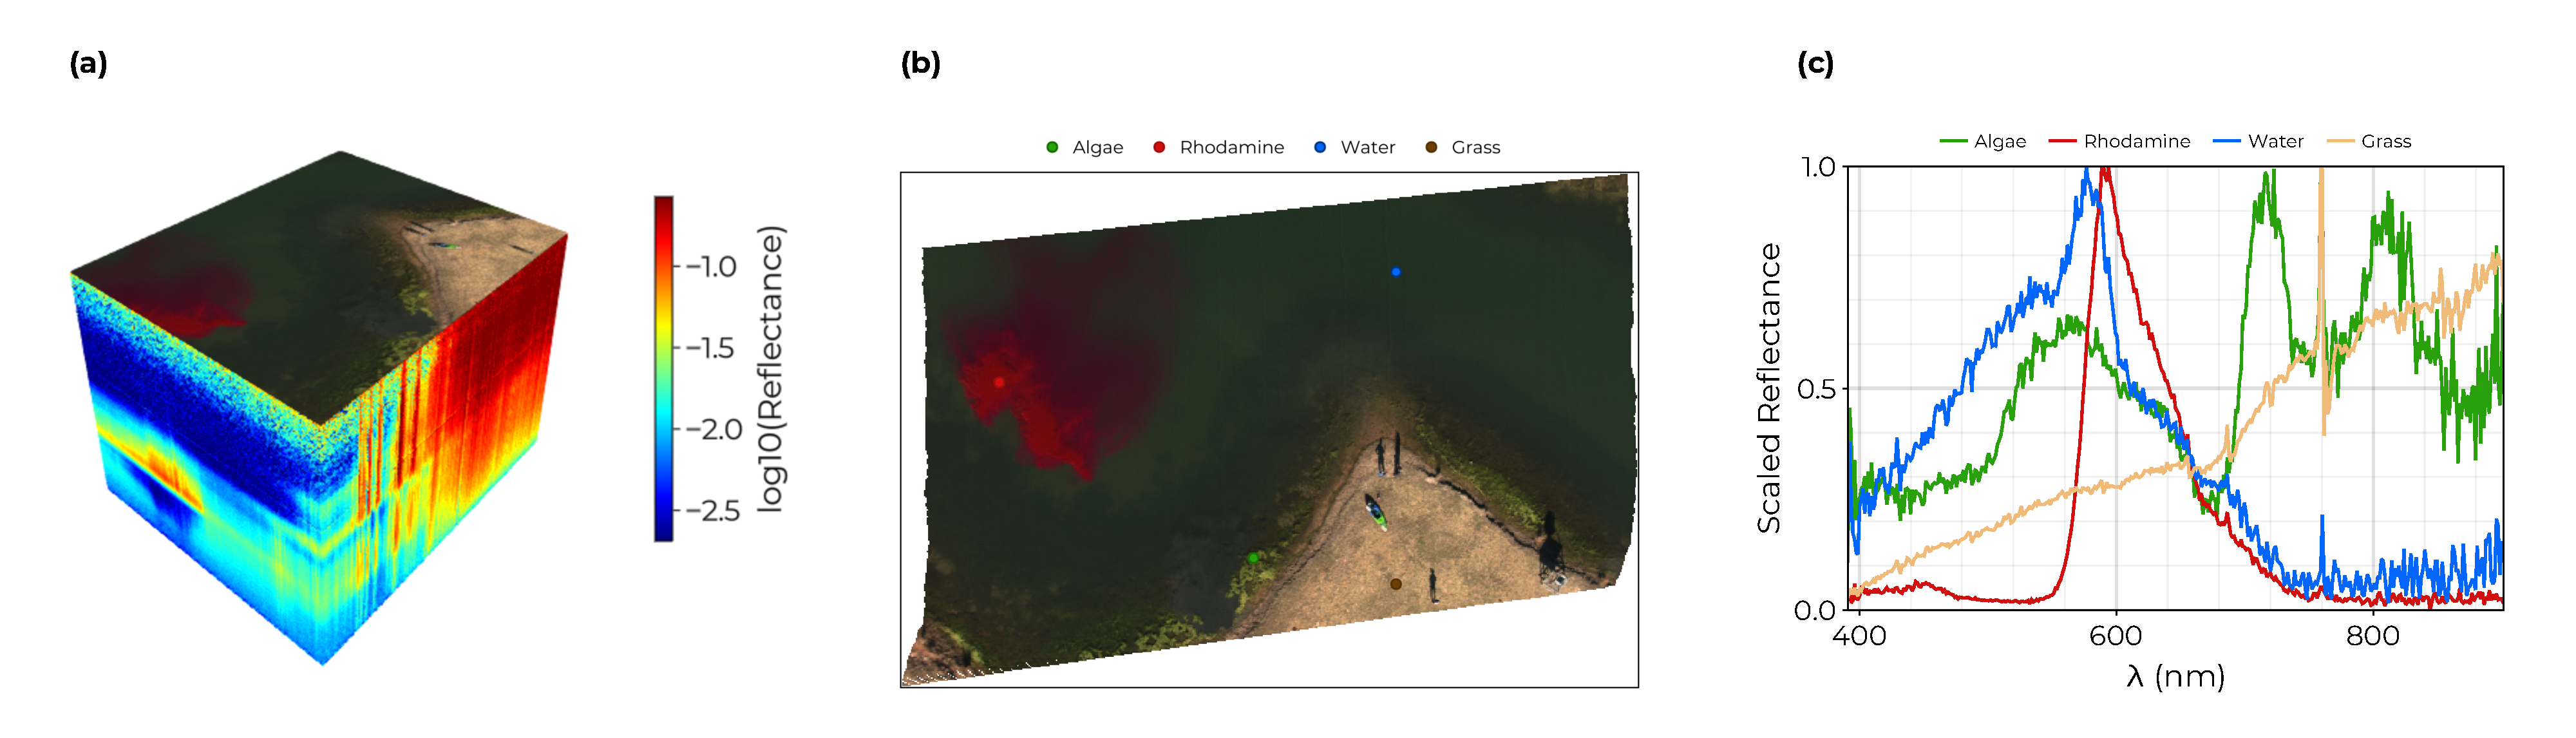
\includegraphics[width=15.5cm]{paper/figures/methods/sample-spectra.pdf}
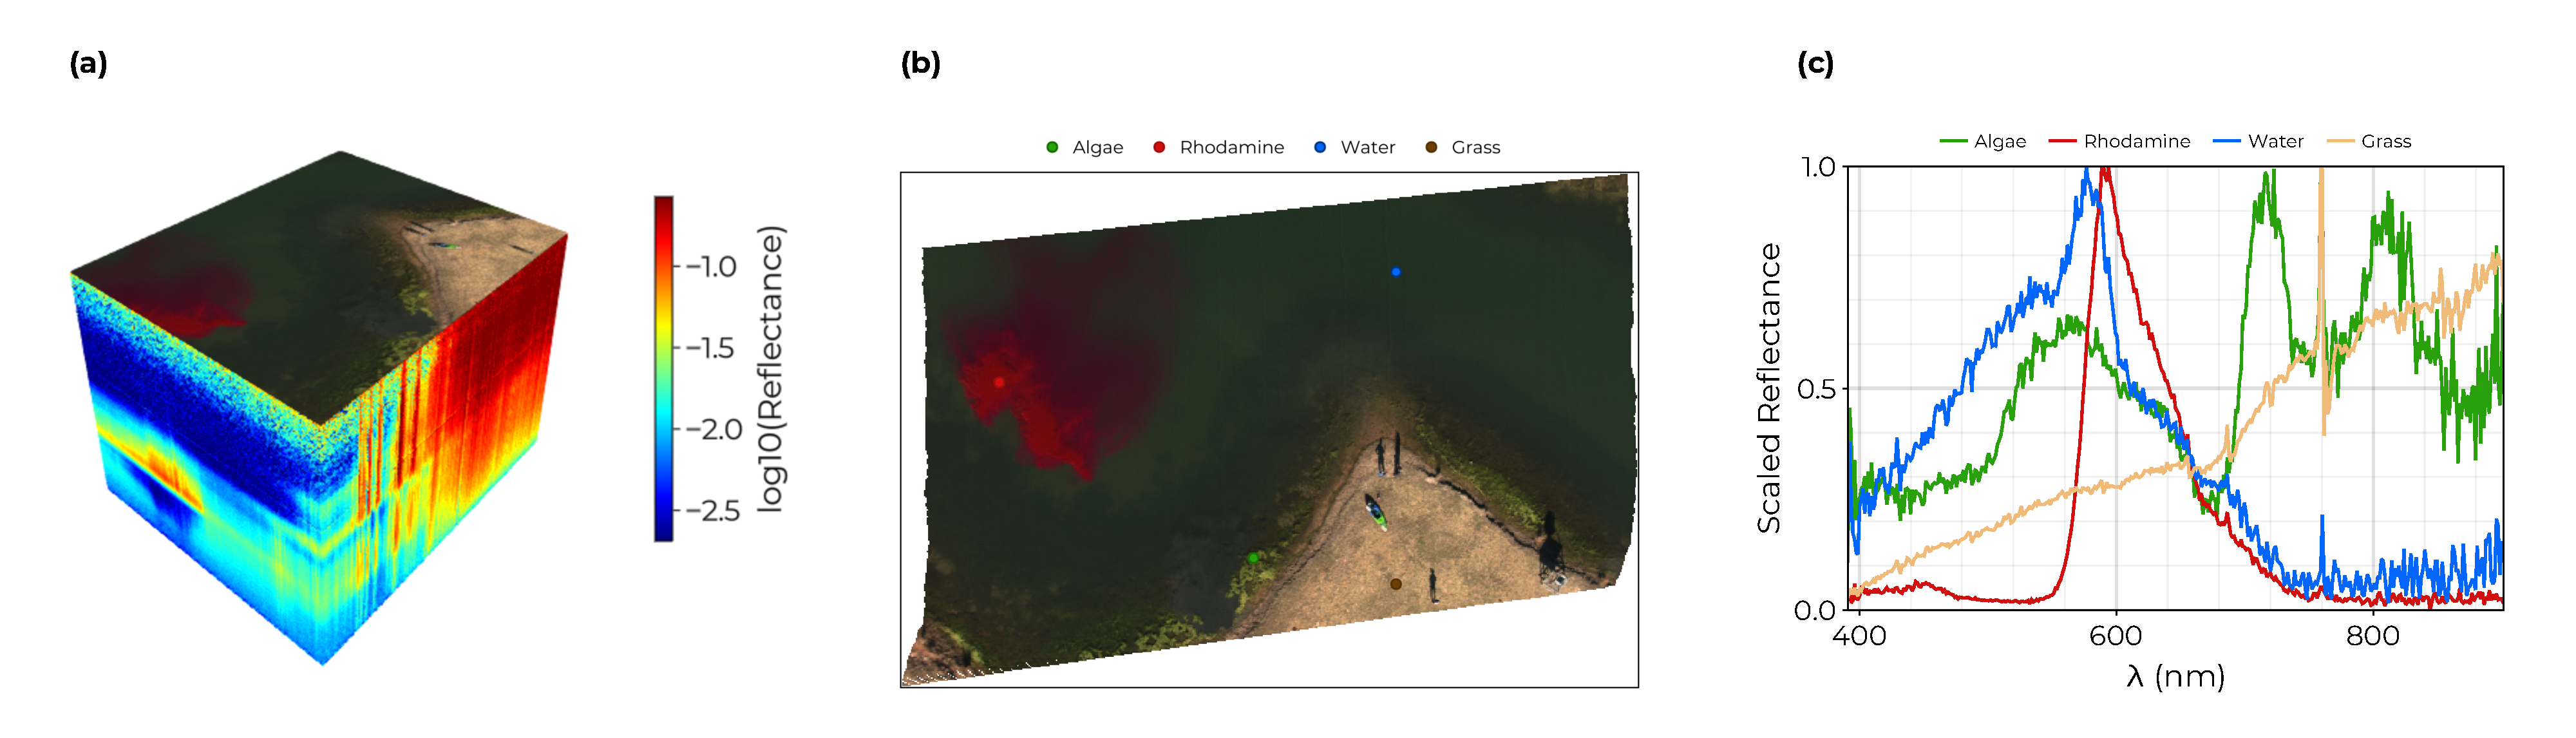
\includegraphics[width=\columnwidth]{paper/figures/methods/sample-spectra.pdf}
%\end{adjustwidth}
\caption{(\textbf{a}) Sample hyperspectral data cube. Spectra are plotted using their geographic position with the log10-reflectance colored along the z axis and a pseudo-color image on top. (\textbf{b}) Points taken from a sample hyperspectral data cube corresponding to algae, rhodamine dye, water, and dry grass. (\textbf{c}) Reflectance spectra for the exemplar points scaled so the peak value of each spectrum is $1.0$. (\textbf{d}) The location of the pond in Montague, Texas where data were collected for this study.\label{fig:sample-spectra}}
\end{figure}  


In this study, we explore the use of the GTM as a tool for dimensionality reduction and non-linear endmember extraction of hyperspectral imagery. To this end, a dataset of HSI were collected at a pond in Montague, North Texas (shown in panel d of Fig~\ref{fig:sample-spectra}) on 23 November 2020 using a UAV mounted hyperspectral imager configured as described in \cite{robot-team-1, robot-team-2}. In this section we first provide a detailed overview of the GTM algorithm. Next we describe the UAV platform used for HSI collection and the various steps used to processes captured HSI. Finally, we describe the two case studies presented in this paper for the utilization of the GTM as a HSI visualization tool and as an endmember extraction technique.

%%% --- Generative Topographic Mapping ------------------------------------
\subsection{Generative Topographic Mapping}\label{sec:gtm-overview}


The GTM is a probabilistic latent variable model inspired by the SOM for visualizing and clustering high-dimensional data. Like the SOM, the GTM assumes vectors $\mathbf{x}$ in the $d$-dimensional data space (here representing reflectance spectra) are constrained to a low-dimensional embedded manifold. The SOM describes this manifold using a regular grid of nodes, each having an associated weight vector defining the mapping from the manifold to the data space. The position of each data record $\mathbf{x}$ in the manifold is assigned to the position of the node whose weight vector has the minimum Euclidean distance to $\mathbf{x}$. An iterative training procedure updates the weight vectors of each node to fit the manifold to the data such that nodes near each other in the SOM grid correspond to similar records in the data space.

The GTM mimics the grid of the SOM by assuming data are generated from latent variables $\xi$ which are constrained to the $K$-many nodes of a regular grid. This assumption corresponds to establishing a prior distribution on the latent space of the form
\begin{equation}\label{eq:latent-prob}
    p(\xi) = \frac{1}{K}\sum_k^K \delta(\xi - \xi_k)
\end{equation}
where $\delta(\cdot)$ is the Dirac delta function.

Points $\xi$ in this latent space are mapped to the embedded manifold by a non-linear function $\psi$ parameterized by weights $W$ as illustrated in Fig~\ref{fig:gtm-diagram}. However, since real data is rarely noise-free, this embedded manifold will not be perfectly thin. To account for this, the points $\xi$ are described in the data space by a radially symmetric Gaussian distribution, $\mathcal{N}(\psi(\xi),\, \beta^{-1})$, with mean $\psi(\xi)$ and variance $\beta^{-1}$. For a dataset $\left\{ \mathbf{x}_n\right\}\limits_{n=1}^N$ consisting of $N$-many i.i.d. records, this choice yields a log-likelihood function of the form
\begin{equation}\label{eq:llh}
    \mathcal{L}(W, \beta) = \sum_n^N \ln \left(\dfrac{1}{K}\sum_k^K p(\mathbf{x}_n \mid \xi_k, W, \beta) \right)
\end{equation}
which can be maximized to yield optimal $W$ and $\beta^{-1}$.

\begin{figure}[t]
%\begin{adjustwidth}{-\extralength}{0cm}
\centering
%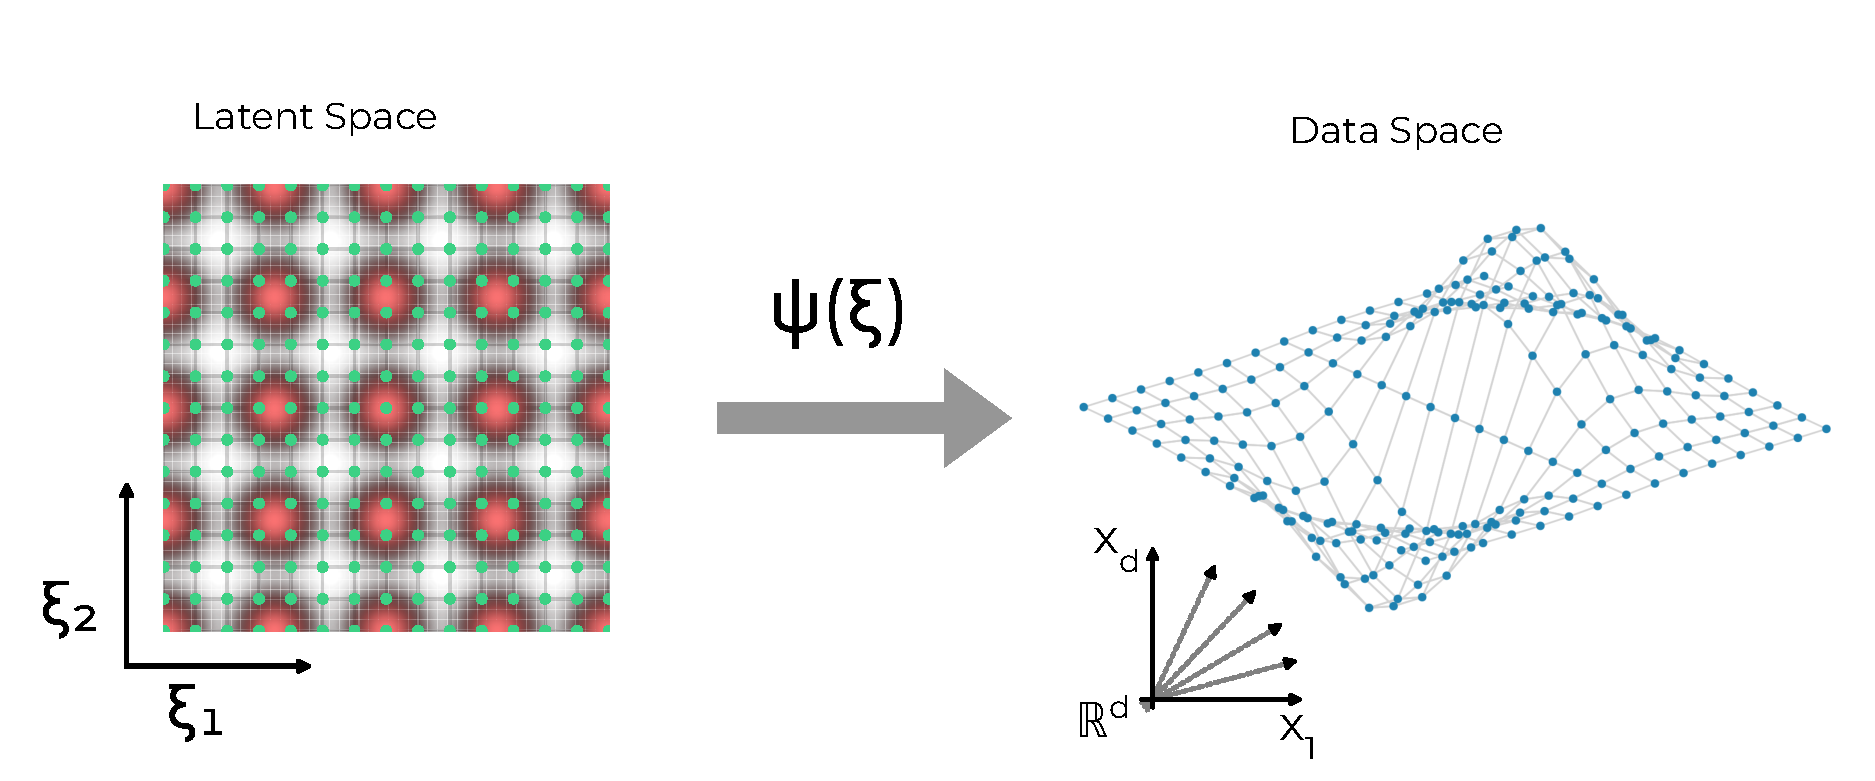
\includegraphics[width=\columnwidth]{paper/figures/methods/gtm-diagram.pdf}
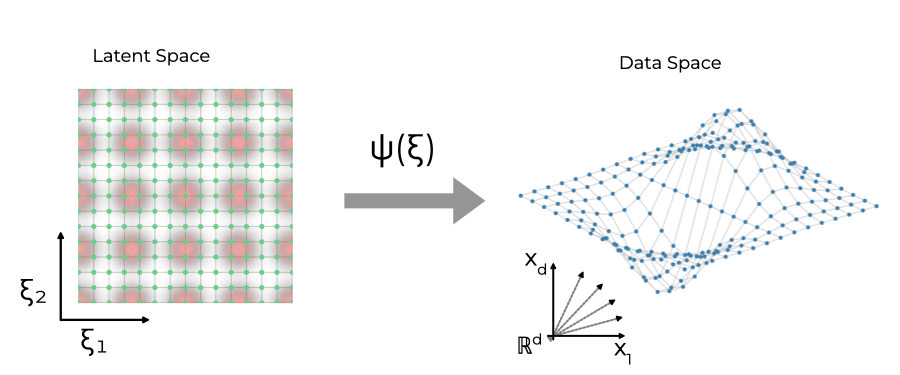
\includegraphics[width=\columnwidth]{paper/figures/methods/gtm-diagram.png}
%\end{adjustwidth}
\caption{Illustration of the GTM algorithm. On the left is a regular grid of $K$ many points (green) in the latent space represented by their coordinates $\xi_1$ and $\xi_2$. In red are the $M$-many RBF which define the mapping $\psi$ from the latent space to the data space. Points in the latent space are mapped non-linearly to the data space yielding an embedded manifold in $\mathcal{R}^d$, here illustrated in three dimensions.\label{fig:gtm-diagram}}
\end{figure}  


The function $\psi$ is typically chosen to be given by the sum of $M$-many radial basis functions (RBF) evenly distributed in the latent space such that $\psi(\xi) = W\phi(\xi)$ with centers $\mu_m$ and width $\sigma$ so that
\begin{equation}
    \phi_m(\xi) = \exp\left(-\dfrac{\lVert \xi - \mu_m \rVert^2}{2\sigma^2}\right).
\end{equation}
The width $\sigma$ is taken as the distance between neighboring RBF centers adjusted by a scale factor labelled $s$. to Together the number of RBFs, $M$, and $s$ are hyperparameters for the model which govern the smoothness of the resulting manifold in the data space. Additionally, sparsity of $W$ can be enforced by introducing an additional hyperparameter $\alpha$ corresponding to a prior distribution over the weights given by
\begin{equation}\label{eq:weight-prior}
    p(W \mid \alpha) =  \left( \frac{\alpha}{2\pi} \right)^{MD/2}\exp\left(-\frac{\alpha}{2}\left\lVert W \right\rVert_{F}^2\right).
\end{equation}

The use of RBFs for $\psi$ enables maximizing $\mathcal{L}(W,\beta)$ via an Expectation-Maximization routine. During each step of the fitting process, the responsibility of the $k$th node for the $n$th data record is computed as 
\begin{equation}\label{eq:responsibility}
    R_{kn} = p(\xi_k \mid \mathbf{x}_n, W, \beta) = \dfrac{p(\mathbf{x}_n \mid \xi_k, W, \beta)}{\sum\limits_{k'}^{K} p(\mathbf{x}_n \mid \xi_{k'}, W, \beta)}.
\end{equation}
Together these responsibilities form a matrix with entries $R_{kn}$ which are kept fixed during the maximization step. The maximization step is then performed by updating the weights $W$ and variance $\beta^{-1}$ according to
\begin{align}\label{eq:m-step}
    W_{\text{new}} &= \left(\Phi^T G \Phi + \dfrac{\alpha}{\beta}I \right)^{-1} \Phi^T R X  \\
    \frac{1}{\beta_{\text{new}}} &= \frac{1}{ND} \sum\limits_{n}^{N} \sum\limits_{k}^{K} R_{kn} \left\lVert \psi_k - \mathbf{x}_n \right\rVert^2
\end{align}
where $\Phi_{km} = \phi_m(\xi_k)$, $X$ is the data matrix formed by concatenating the records $\mathbf{x}_n$, and $G$ is a diagonal matrix with $G_{kk} = \sum\limits_n^N R_{kn}$. This process is repeated until the log-likelihood converges to a predetermined tolerance level.

Slices $R_{[:,n]}$ of the matrix $R$ define the responsibility of each latent node $\xi_k$ for the $n$th data record $\mathbf{x}_n$. Therefore the final responsibility matrix after GTM training can be used to represent each record in the latent space by the mean:
\begin{equation}
    \hat{\xi}_n = \sum_{k}^K R_{kn}\xi_k.
\end{equation}

A freely available implementation of the GTM algorithm was developed for this study and is accessible at \cite{gtm-code}. The code is written in the Julia programming language and complies with the Machine Learning in Julia (MLJ) common interface \cite{bezanson2012julia,blaom2020mlj}.

\subsection{UAV-Based Hyperspectral Imaging}

A Freefly Alta-X autonomous quadcopter was used as the UAV platform in this study. This UAV was equipped with a Resonon Pika XC2 visible+near-infrared (VNIR) hyperspectral imager to capture HSI with $462$ wavelengths per pixel ranging from $391$ to $1011$ nm. This imager is in a pushbroom configuration so that HSI are captured one scan-line at a time resulting in data cubes consisting of $1000$ scan-lines with $1600$ pixels each. Additionally, the camera includes an embedded GPS/INS unit to enable georectification of collected HSI. An upward facing Ocean Optics UV-Vis NIR spectrometer with a cosine corrector was also included to provide measurements of the incident solar irradiance spectrum. The configuration of the UAV with the attached hyperspectral imager is shown in Fig~\ref{fig:drone}. Data collection and processing was controlled by an attached Intel NUC small-form-factor computer.

To account for the variability of incident light, raw HSI are converted to units of reflectance using the downwelling irradiance spectrum simultaneously captured with each HSI. With the hyperspectral imager oriented to nadir, the reflectance is given by
\begin{equation}\label{eq:reflectance}
    R(\lambda) = \pi L(\lambda)/E_d(\lambda)
\end{equation}
where $L$ is the spectral radiance, $E_d$ is the downwelling irradiance, and a factor of $\pi$ steradians results from assuming the water surface is Lambertian (diffuse) \cite{ruddick2019review}. HSI collection was performed near solar noon to maximize the amount of incident sunlight illuminating the water. For the site in North Texas, this corresponded to an average solar zenith angle of $54.9^\circ$ for 23 November 2020 resulting in HSI with negligible sunglint effects. 



\begin{figure}[t]
\begin{adjustwidth}{-\extralength}{0cm}
\centering
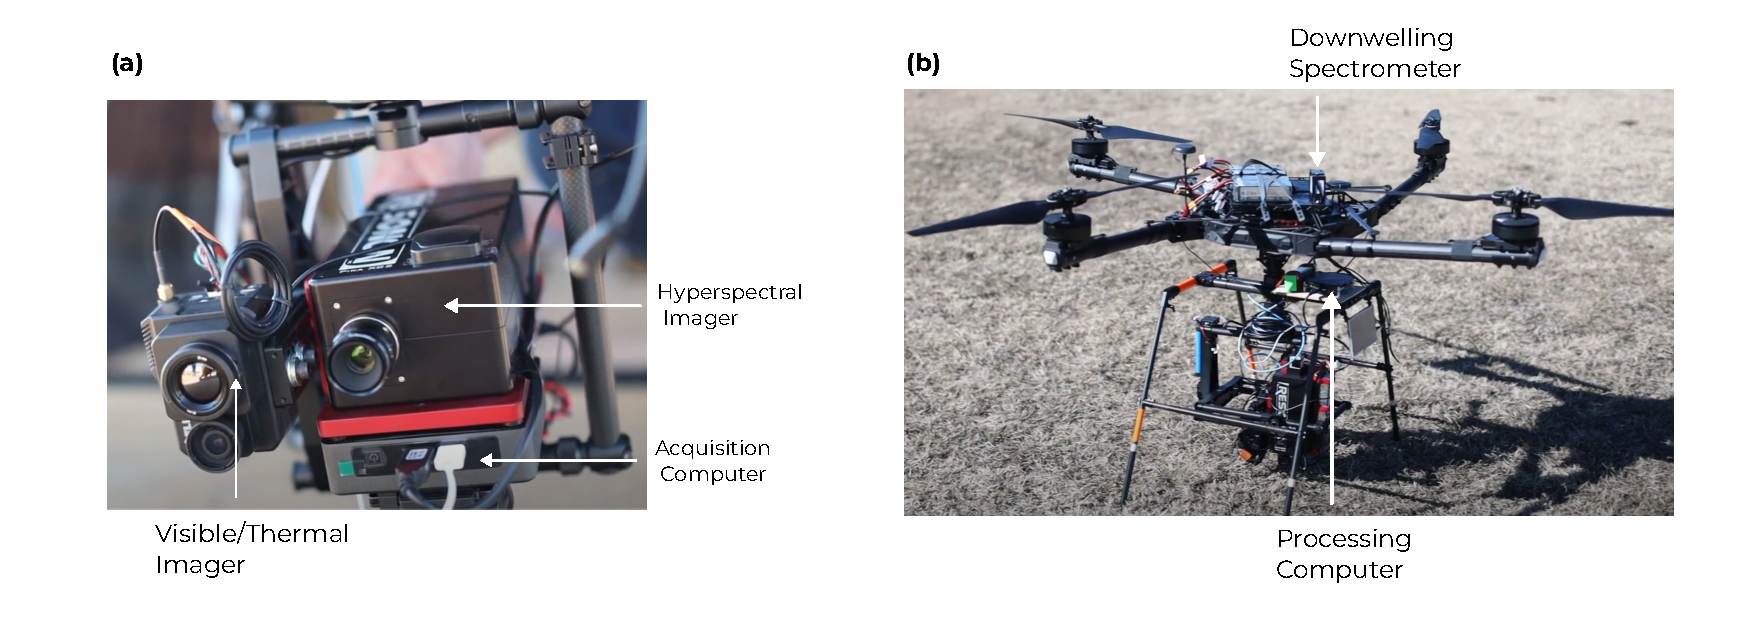
\includegraphics[width=15.5cm]{paper/figures/methods/annotated-drone.pdf}
\end{adjustwidth}
\caption{The UAV platform: (\textbf{a}) The Resonon Pika XC2 hyperspectral imager. (\text{b}) The Freefly Alta-X with the attached hyperspectral imager, processing computer, and downwelling irradiance spectrometer. \label{fig:drone}}
\end{figure}  




After conversion to reflectance, each HSI must also be georectified to assign geographic coordinates to each pixel. The UAV flights were performed at an approximate altitude of $50$ m above the water so that the imaging surface can be considered to be flat. Consequently, HSI were rapidly georectified to a $10$ cm resolution using position and orientation data from the embedded GPS/INS as outlined in \cite{muller2002program, baumker2001new, mostafa2000multi}. An example hyperspectral data cube is illustrated in panel (a) of Fig~\ref{fig:spectral-signatures} where the log10-reflectance values are plotted along the z-axis for each pixel in the scene and a psuedo-color image at the top of the data cube illustrates how the water would appear to the human eye from the perspective of the UAV.

As a final processing step before training each GTM, we limit the wavelengths of each HSI to $\lambda \leq 900$ nm as wavelengths above $900$ nm showed significant noise. Additionally, each spectrum was re-scaled to a peak value of $1.0$ to account for incident light variability between HSI.

\subsection{GTM Case Studies}\label{sec:case-studies}

To explore the ability of the GTM to segment HSI pixels and aid in source identification we first consider a dataset of water-only spectra consisting of $>36,000$ records identified from collected HSI by a normalized difference water index (NDWI) greater than $0.25$ where the NDWI is defined as 
\begin{equation}
    \text{NDWI} = \dfrac{R(550) - R(860)}{R(550) + R(860)}.
\end{equation}
We then apply the trained GTM to all water-only pixels to visualize the distribution learned by the GTM and examine spectra associated with a subset of nodes in the latent space in order to assess the small-scale spatial variability within the pond.

Next, we consider a dataset of combined HSI pixels including both water and land. To simulate the dispersion of a potential contaminant source, a Rhodamine tracer dye was released into the western portion of the pond and two additional UAV flights were used to collect HSI capturing the evolution of the resulting plume. From these HSI a collection of $>145,000$ were sampled for model training. Exemplar spectra for water, grass, algae, and rhodamine dye were identified from a sample HSI as shown in panels (b) and (c) of Fig~\ref{fig:sample-spectra}. Using these spectra, we explore the trained GTM and use it to extract spectral signatures corresponding to these endmember categories. Values for the hyperparameters $m$, $s$, and $\alpha$, are determined by training multiple GTM models and selecting values which minimize the Bayesian Information Criterion (BIC) given by 
\begin{equation}
    \text{BIC} = 2P\ln(N) - 2\mathcal{L}
\end{equation}
where $P$ is the total number of model parameters, $N$ is the number of records in the dataset, and $\mathcal{L}$ is the log-likelihood defined in Eq~\ref{eq:llh}.

The normalized spectral similarity score (NS3) introduced by Nidamanuri and Zbell combines the root-mean-square (RMS) difference together with the spectral angle to provide a spectral distance function\cite{nidamanuri2010normalized}. For two spectra $R_1(\lambda)$ and $R_2(\lambda)$ it is defined by
\begin{equation}
    \text{NS3}(R_1, R_2) &= \sqrt{RMS(R_1, R_2)^2 + (1-\cos\theta)^2}
\end{equation}
where
\begin{align}
    \text{RMS}(R_1, R_2) &= \sqrt{\frac{1}{N-1}\sum_\lambda \left(R_{1}(\lambda) - R_2(\lambda) \right)^2} \\
    \cos\theta &= \frac{\langle R_1 , R_2 \rangle}{\lVert R_1\rVert \lVert R_2 \rVert}.
\end{align}
We use the NS3 together with identified spectral endmembers to map the abundance of algae near the shore as well as the evolution of the Rhodamine dye plume.

%%%%%%%%%%%%%%%%%%%%%%%%%%%%%%%%%%%%%%%%%%
\section{Results}

\subsection{Water-only Pixel Segmentation}

\begin{figure}[t]
\begin{adjustwidth}{-\extralength}{0cm}
\centering
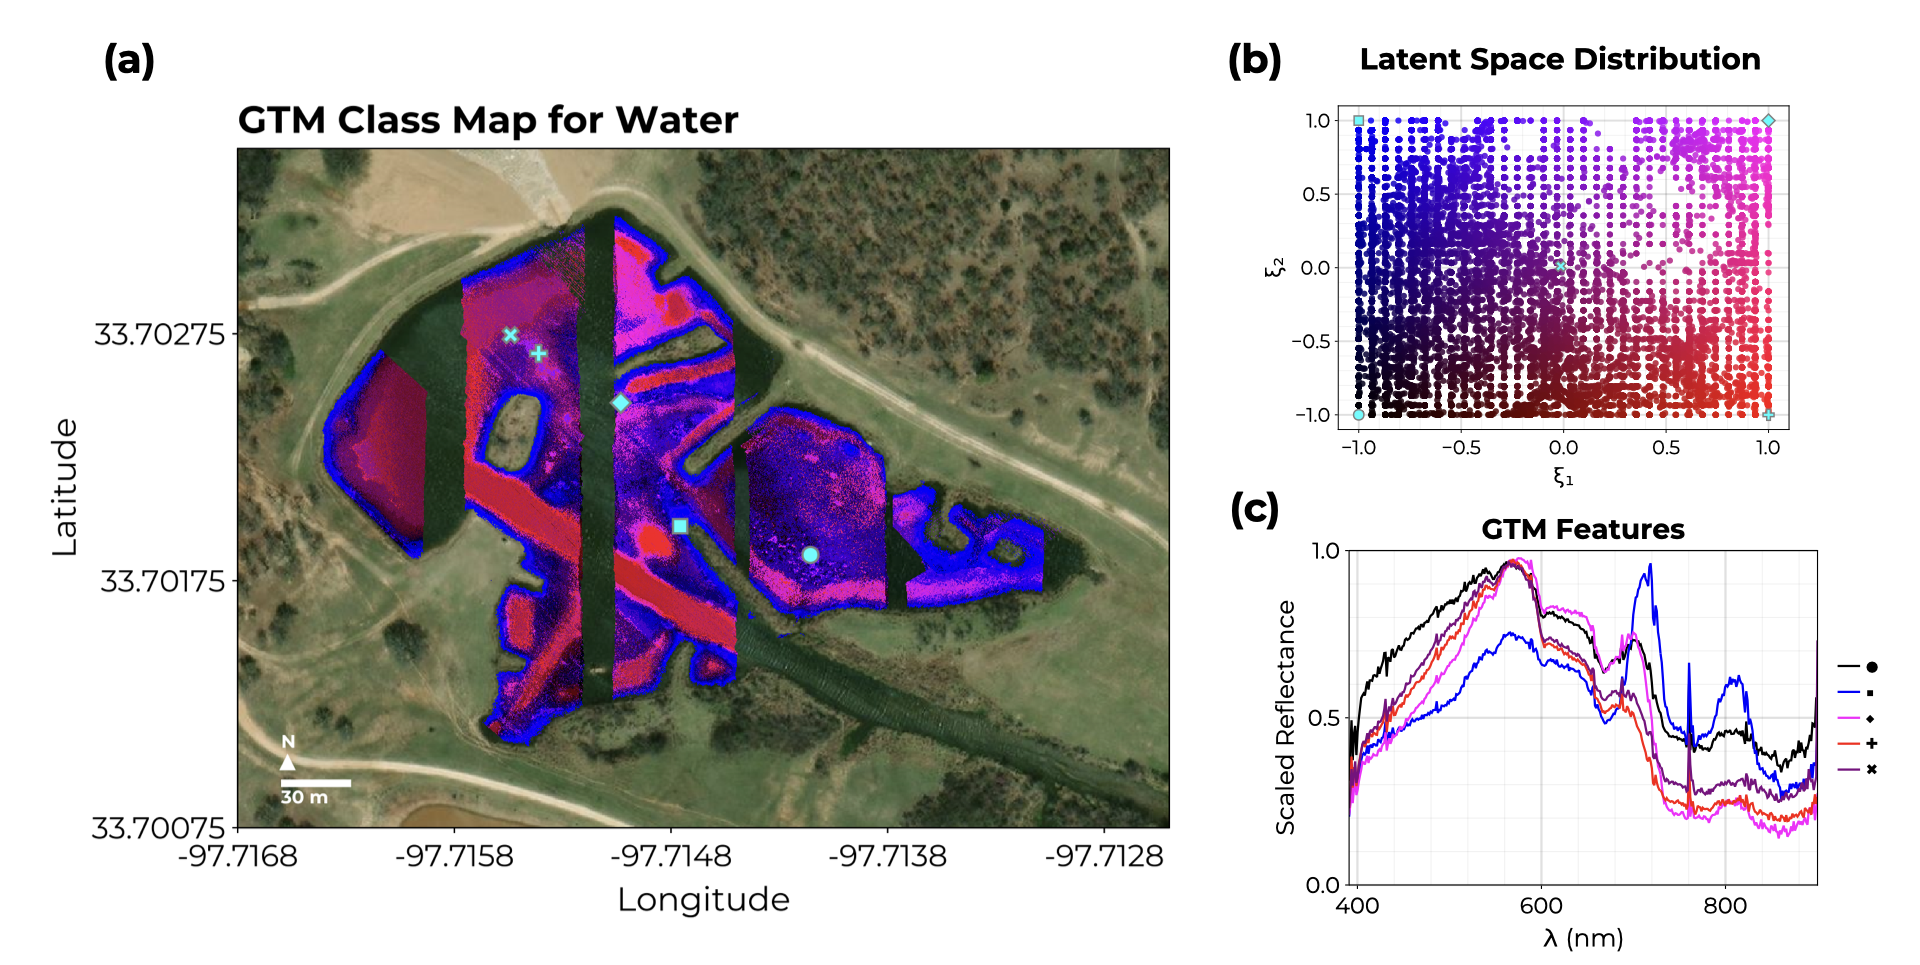
\includegraphics[width=18.0cm]{paper/figures/results/gtm-water.png}
\end{adjustwidth}
\caption{Classification map for GTM trained solely on water pixels (no land and no rhodamine plume). \textbf{(a)} GTM applied to all water pixels colored by their associated position in the latent space. \textbf{(b)} Representation of the points from the training set in the latent space. Color is assigned to each point by mapping $\xi_1$ to red and $\xi_2$ to blue. \textbf{(c)} GTM spectral signatures, $\psi(\xi_k)$, corresponding to nodes from the four corners and center of the GTM latent space. \label{fig:gtm-water}}
\end{figure}  

A GTM with $K=32\times 32$ nodes was trained on the dataset of water-only pixels described in Sec~\ref{sec:case-studies} in order to explore the distribution of reflectance spectra captured by the HSI. The resulting GTM is visualized in Fig~\ref{fig:gtm-water}. First, we note that the GTM has utilized most of the embedding space as illustrated panel (b) where the position corresponding to the mean responsibility of each data point $\hat{\xi}_n$ has been plotted in the latent space. For this water-only gtm, the spectra appear to be largely clustered toward the left edge, bottom, and right edge of the embedding space. Spectral signatures corresponding to GTM nodes from the four corners and center of the latent space are shown in panel (c) illustrating the spectral variability represented across the latent space. 

To visualize the distribution of HSI learned by the GTM, we can associate a color with each dimension of the latent space. In Fig~\ref{fig:gtm-water} we have used the red channel to represent $\xi_1$ and the blue channel to represent $\xi_2$. Applying the trained GTM to compute mean node responsibilities for all water-pixels in collected HSI allows us to illustrate the spatial distribution of the spectra on a map as shown in panel (a). Here we observe a clear distinction between water near the shore and water in the middle of the pond. Additionally, the eastern alcove of the pond is significantly more blue than the rest of the water reflecting the limited flow through this region. The close proximity of highly dissimilar GTM classes illustrated by sharp color gradients in the map captures the small-scale spatial variability typical of inland water bodies like this pond.

\subsection{Endmember Extraction}

\begin{figure}[t]
\centering
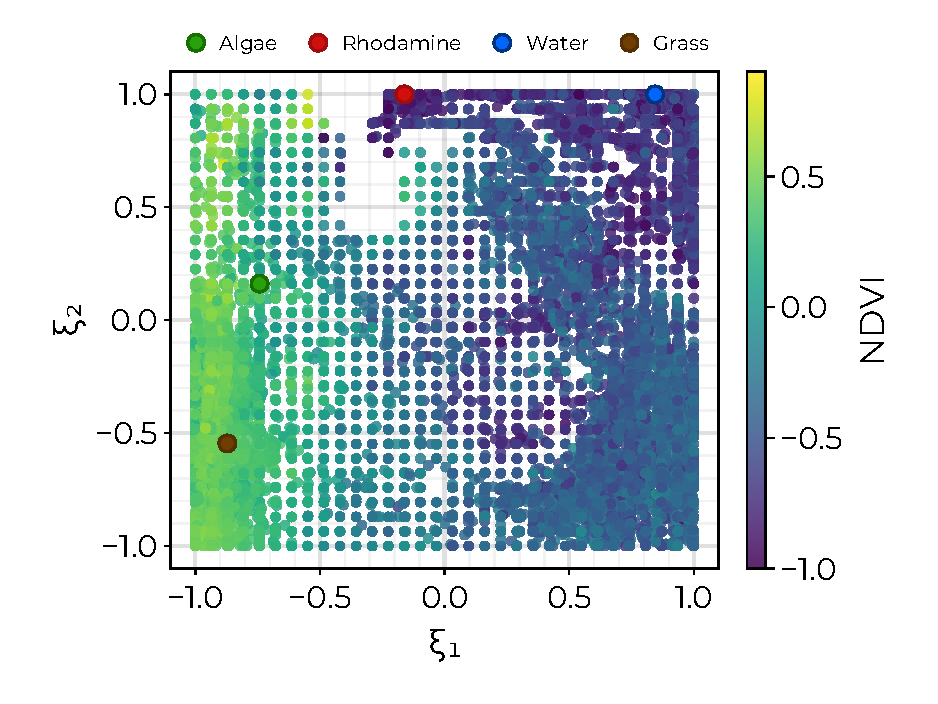
\includegraphics[width=0.8\columnwidth]{paper/figures/results/square-ndvi.pdf}
%\caption{GTM Map: We plot the mean position of each data point in the latent space with points colored by the their associated NDVI values. The locations of the exemplar points for algae, rhodamine dye, water, and dry grass are shown in the latent space illustrating that the GTM has clearly distinguished land, near-land, and water pixels.\label{fig:gtm-ndvi}}
\caption{GTM latent space visualization: Each sample spectrum from the dataset of combined HSI covering shore, water, and the rhodamine dye release are plotted in the GTM latent space at the location of the mean node responsibility, $\hat{\xi}_n$. Points are colored according to the NDVI computed from the original reflectance spectra. The locations of exemplar spectra for algae, rhodamine, water, and grass in the latent space are included as color-filled circles. Spectra from the shore and water are clearly separated to different regions of the latent space.\label{fig:gtm-ndvi}}
\end{figure}  

A second GTM was trained on the combined dataset of HSI covering shore, water, and the rhodamine tracer dye release. The resulting class map is shown in Fig~\ref{fig:ndvi} where each sample has been plotted at the position of the mean node responsibility and colored by the normalized difference vegetation index (NDVI) computed from the original reflectance spectrum. The NDVI is a spectral index sensitive to variations in vegetation health with negative values corresponding to water, small positive values corresponding to sparse vegetation, and large values near $1$ corresponding to dense vegetation \cite{thenkabail2018hyperspectral}. From this, we see that the GTM can clearly separate spectra by vegetation content with high values concentrated to the left of the embedding space and negative, water-based pixels concentrated to the right. Additionally, the position of exemplar spectra for algae, rhodamine, water, and grass are included as color-filled circles further illustrating the classification obtained by the GTM.

%\begin{figure}[t]
\begin{figure}[h]
\begin{adjustwidth}{-\extralength}{0cm}
\centering
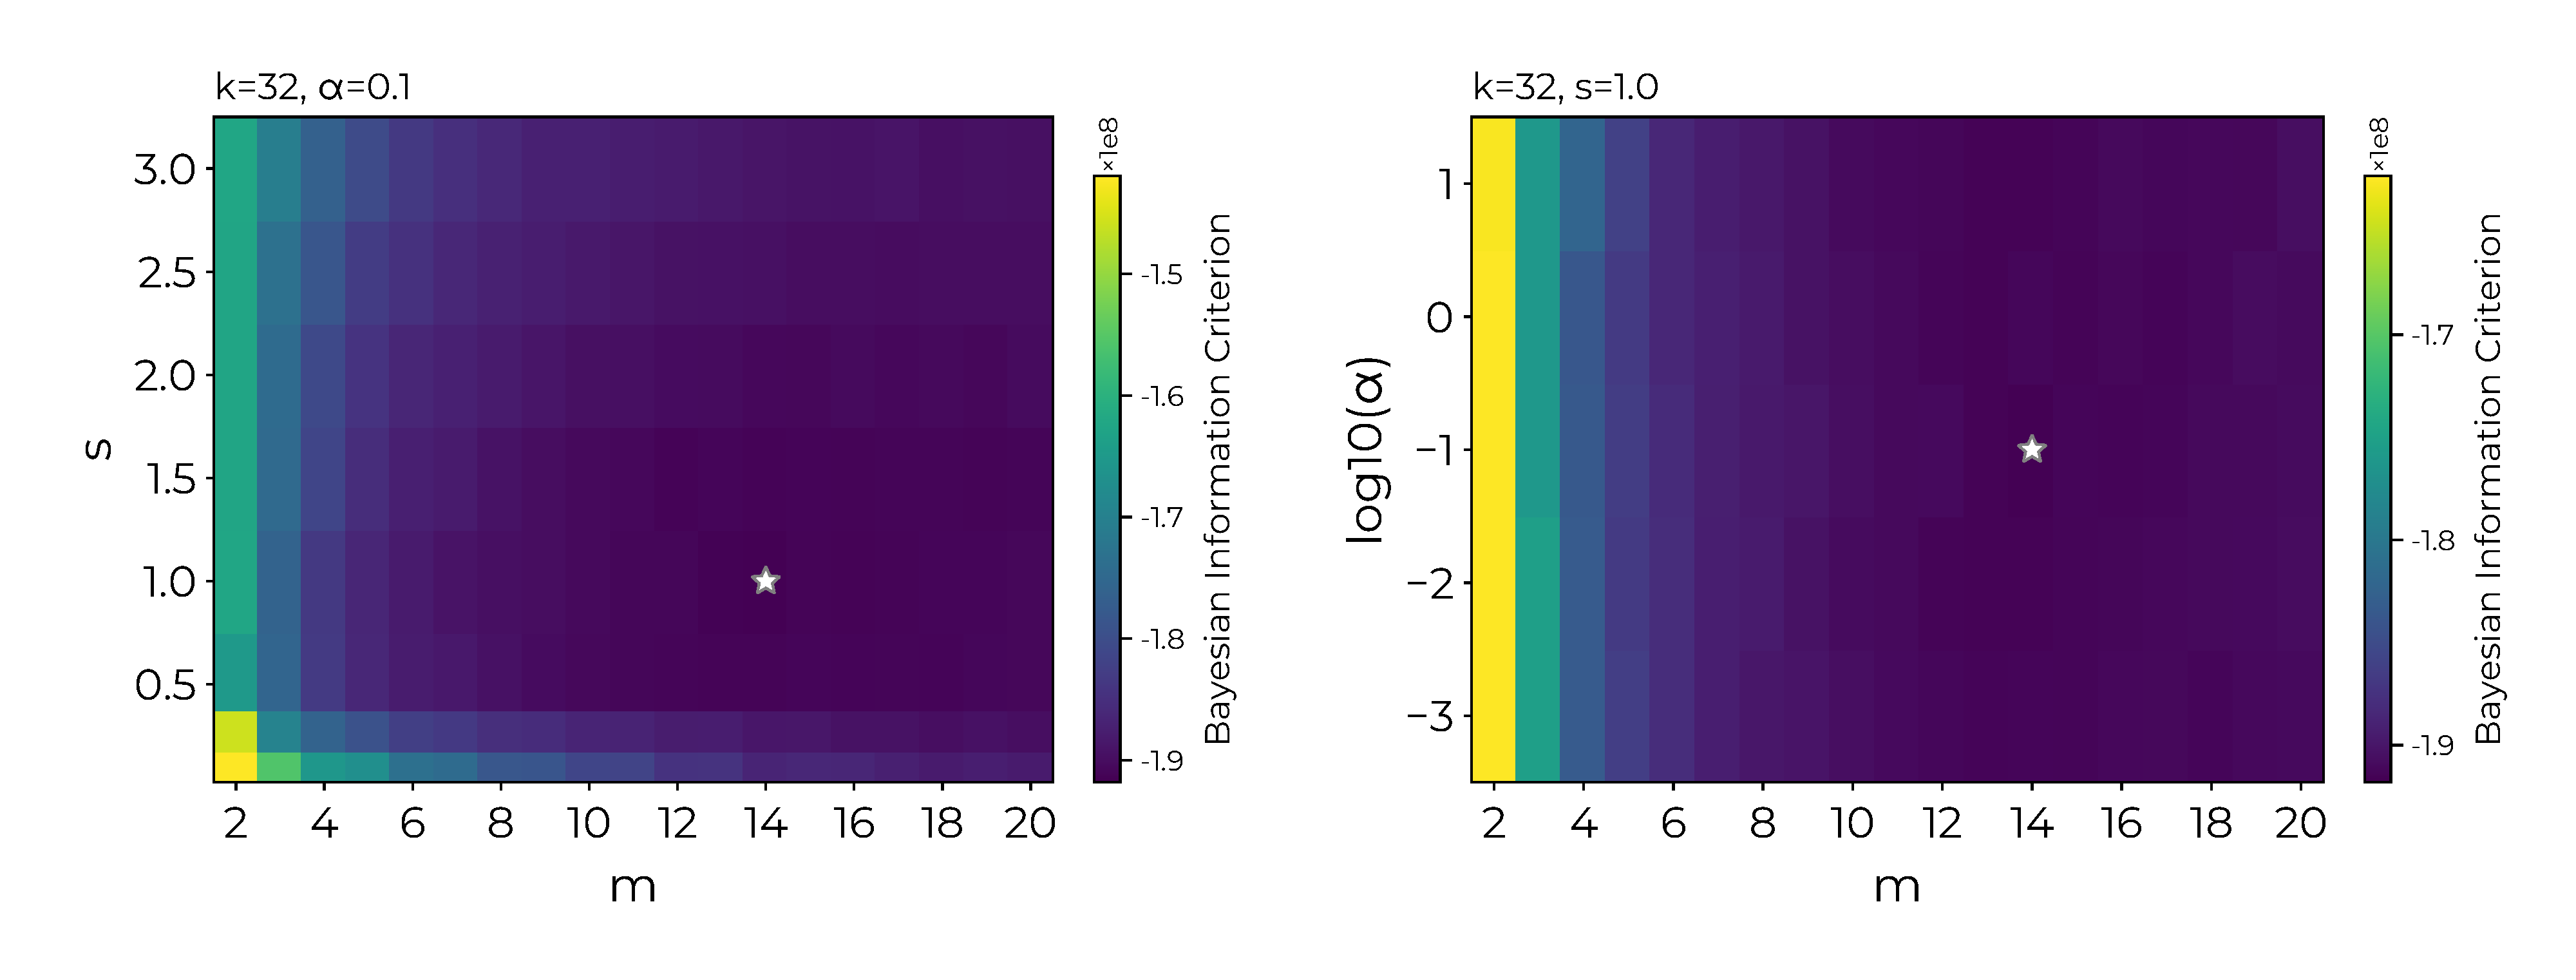
\includegraphics[width=17.0cm]{paper/figures/results/bic.pdf}
\end{adjustwidth}
\caption{Results of the hyperparameter search. (\textbf{left}) Variation of BIC with $m$ and $s$ for fixed $\alpha=0.1$. (\textbf{right}) Variation of the BIC with with $m$ and $\alpha$ for fixed $s=1.0$. The white star in each plot indicates the parameters with the lowest BIC across the entire parameter search.\label{fig:hp-results}}
\end{figure}  

As outlined in Sec~\ref{sec:gtm-overview}, there are three hyperparameters that need to be chosen to fit a GTM model: the number of RBF centers $M=m^2$ with $m$ the number along each axis, the scale factor $s$ which controls the RBF overlap, and the regularization parameter $\alpha$. To choose appropriate values we performed a grid search for $m$ values between $2$ and $20$, $s$ values between $0.1$ and $3.0$, and $\alpha$ values between $0.001$ and $10.0$. The best values were determined as those which minimized the BIC, with $m=14$, $s=1.0$, and $\alpha=0.1$, respectively. Heatmaps comparing the BIC for different hyperparameter values are provided in Fig~\ref{fig:hp-results} and a table of the top 25 models is given in Appendix A.  Since the matrix of RBF activations $\Phi$ need only be computed once at the GTM initialization step, the number of latent nodes given by $K=k^2$ can be chosen to be large enough to ensure a smooth mapping. We found that a value of $k=32$ provided a sufficient number of GTM nodes without significantly impacting training time.

\begin{figure}[t]
\begin{adjustwidth}{-\extralength}{0cm}
\centering
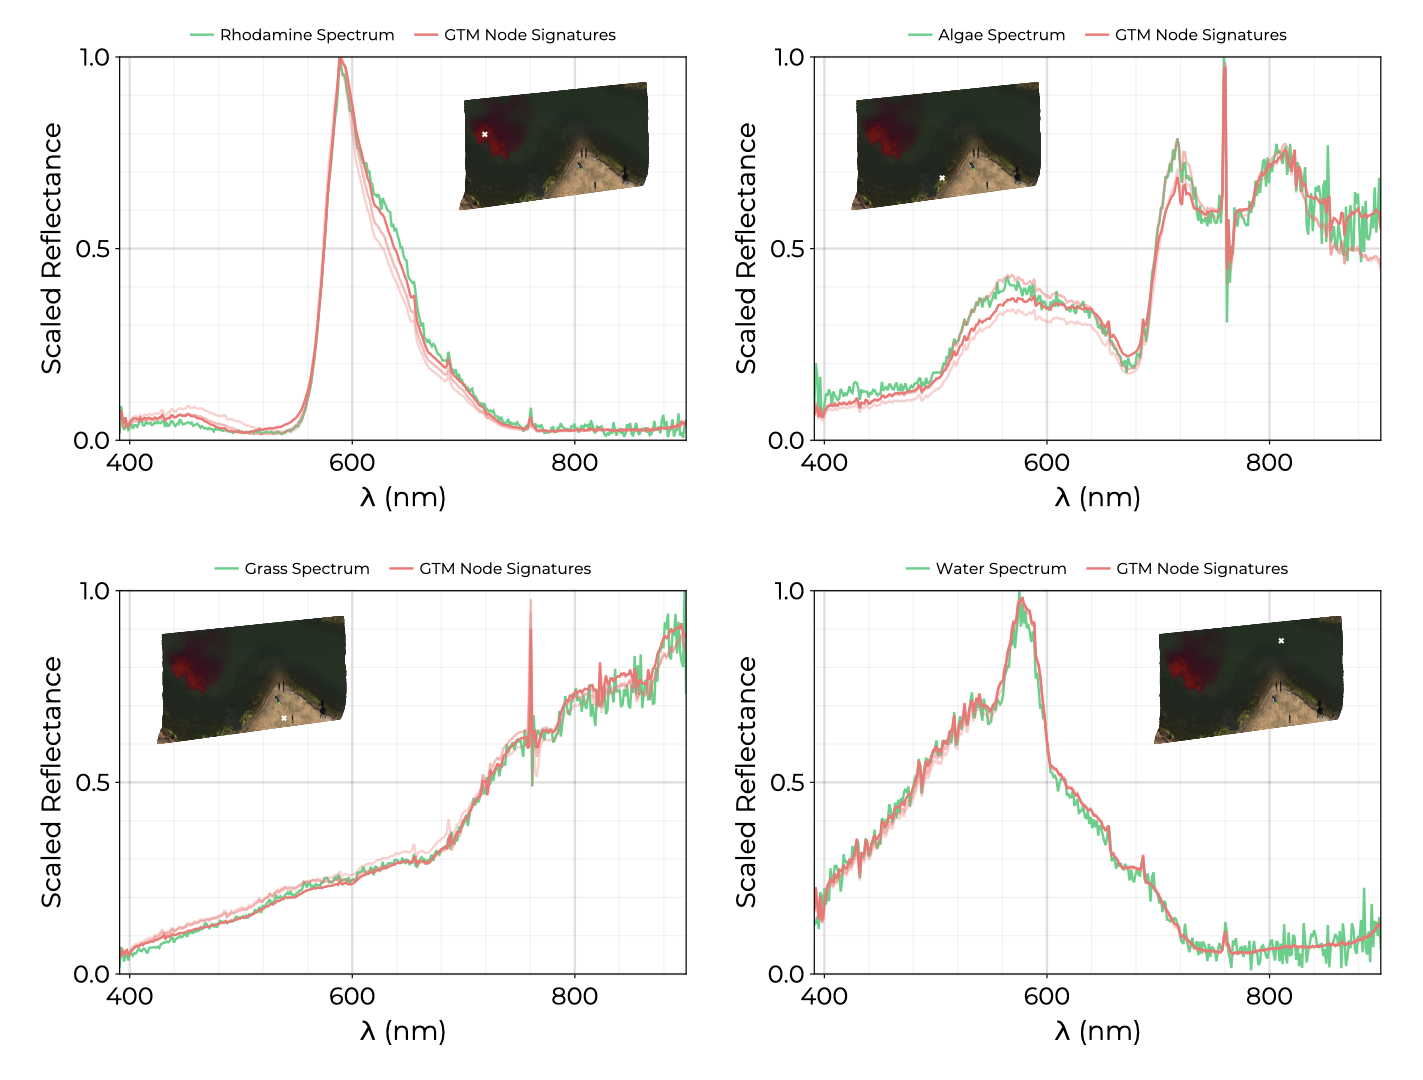
\includegraphics[width=17.0cm]{paper/figures/results/spectral-signatures.png}
\end{adjustwidth}
\caption{Spectral signatures $\psi(\xi_k)$ corresponding to GTM nodes with non-zero responsibility for exemplar spectra corresponding to the rhodamine dye plume (top left), algae (top right), dry grass (bottom left), and open water (bottom right). A pseudo-color image is inset into each plot wit the location of the exemplar spectrum marked with a white circle. \label{fig:spectral-signatures}}
\end{figure}  

Using the trained GTM we can compute spectral signatures for each node in the latent space via the non-linear mapping $\psi$. The responsibilities $R_{kn}$ therefore correspond to the contributions of the $kth$ node $\xi_k$ to the $n$th sample spectrum in the dataset. Endmembers are identified by nodes with non-zero responsibility values for each of the selected exemplar spectra and are plotted in Fig~\ref{fig:spectral-signatures}. We note that these extracted endmembers are able to accurately capture the shape of exemplar spectrum including thin reflectance peaks. The endmembers also manage to smoothly interpolate through noisy wavelengths as shown by the water and algae endmembers for $\lambda > 800$ nm.

\subsection{Abundance Mapping with NS3}

\begin{figure}[t]
\begin{adjustwidth}{-\extralength}{0cm}
\centering
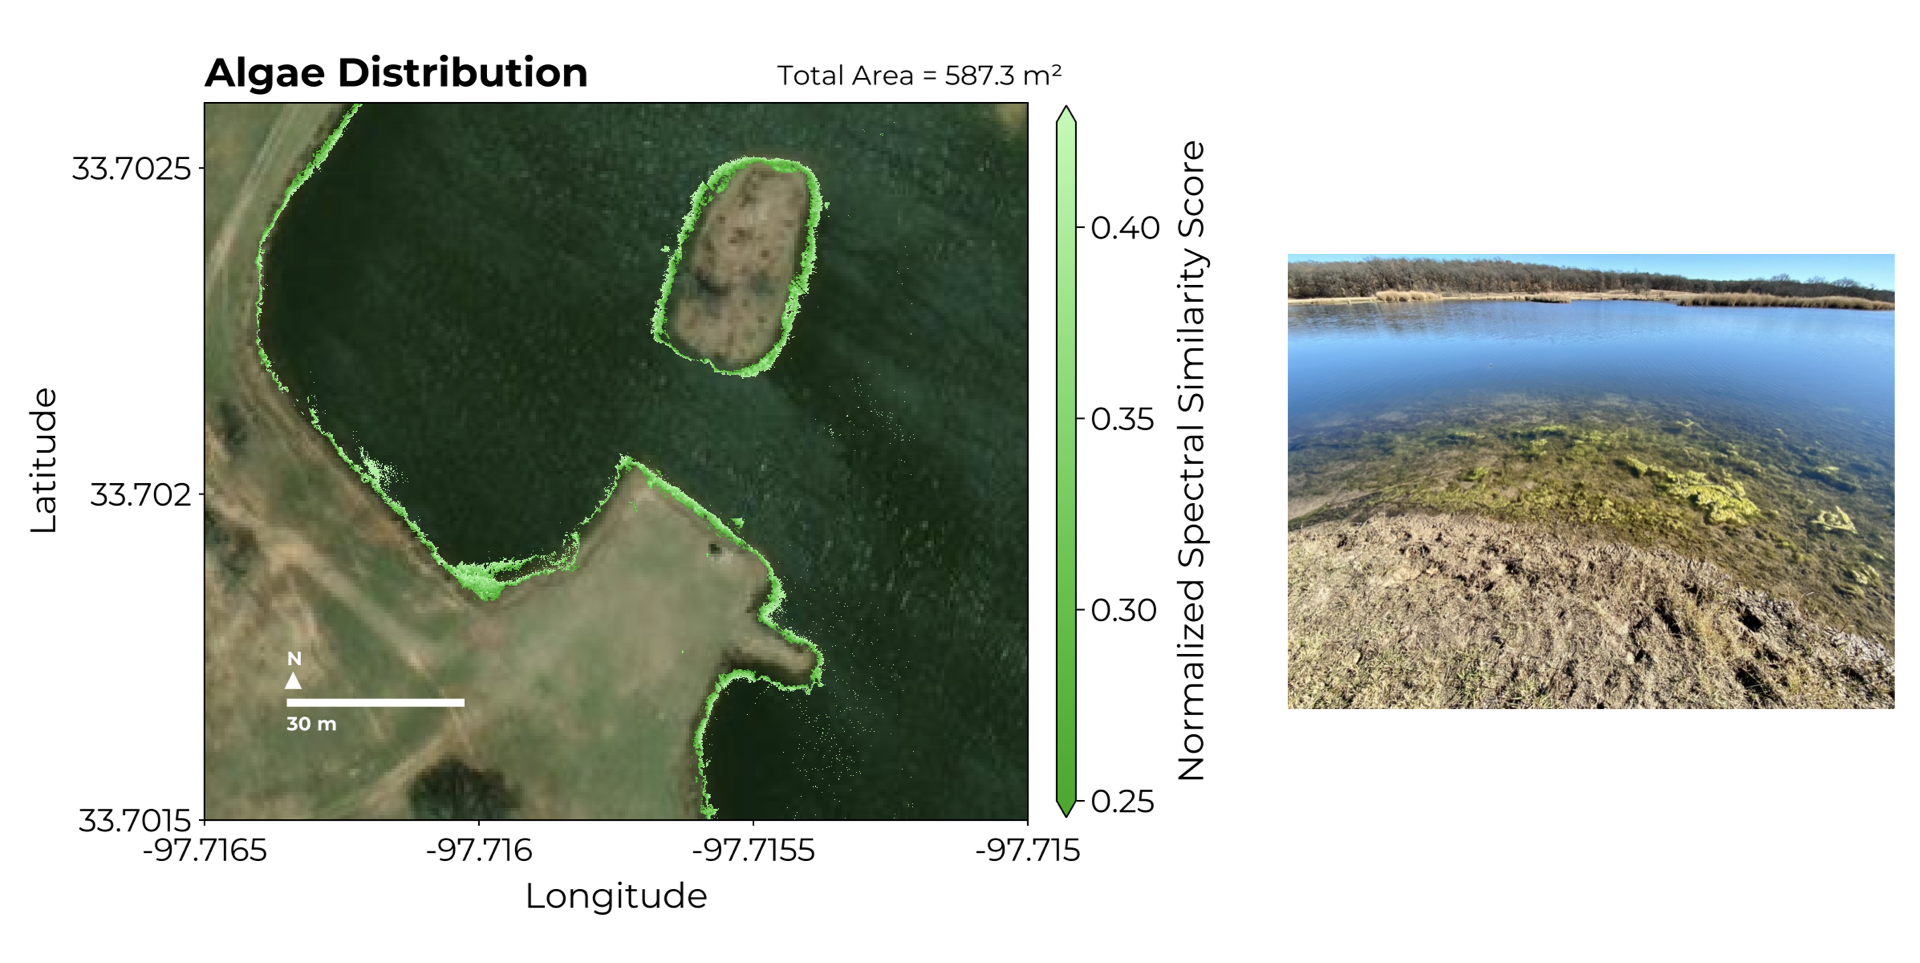
\includegraphics[width=17.0cm]{paper/figures/results/algae.png}
\end{adjustwidth}
\caption{Using the spectral endmember assigned to algae from the trained GTM together with the NS3, we are able to estimate the algal abundance near the shore. (\textbf{left}) NS3 values of pixels below a threshold of 0.4275 corresponding to a total area of $587.3$ $m^2$. (\textbf{right}) A picture of the pond near the shore showing the algae.\label{fig:algae-map}}
\end{figure}  

Spectral endmembers extracted from the GTM can be used to map the abundance of water constituents in HSI by selecting HSI pixels with a NS3 value below a given threshold. In Fig~\ref{fig:algae-map} we demonstrate this by using the extracted algae endmember spectrum to map algal abundance near the western shore of the pond. Identifying algae pixels as those with an NS3 value below 0.4725, we estimate the area subsumed by algae in Fig~\ref{fig:algae-map} to be $587.3$ $m^2$. Similarly, we are able to track the evolution of the rhodamine dye release into the western portion of the pond by computing the NS3 for HSI collected across multiple flights. In the left panel of Fig~\ref{fig:rhodamine-map}, we see that the dye plume initially encompasses an area of roughly $330.7$ $m^2$. A second flight performed 15 minutes later reveals the dye plume to have increased to an area of $1495.6$ $m^2$. The increase in NS3 values between flights reflects the dilution of dye as it diffused into the water.




\begin{figure}[t]
\begin{adjustwidth}{-\extralength}{0cm}
\centering
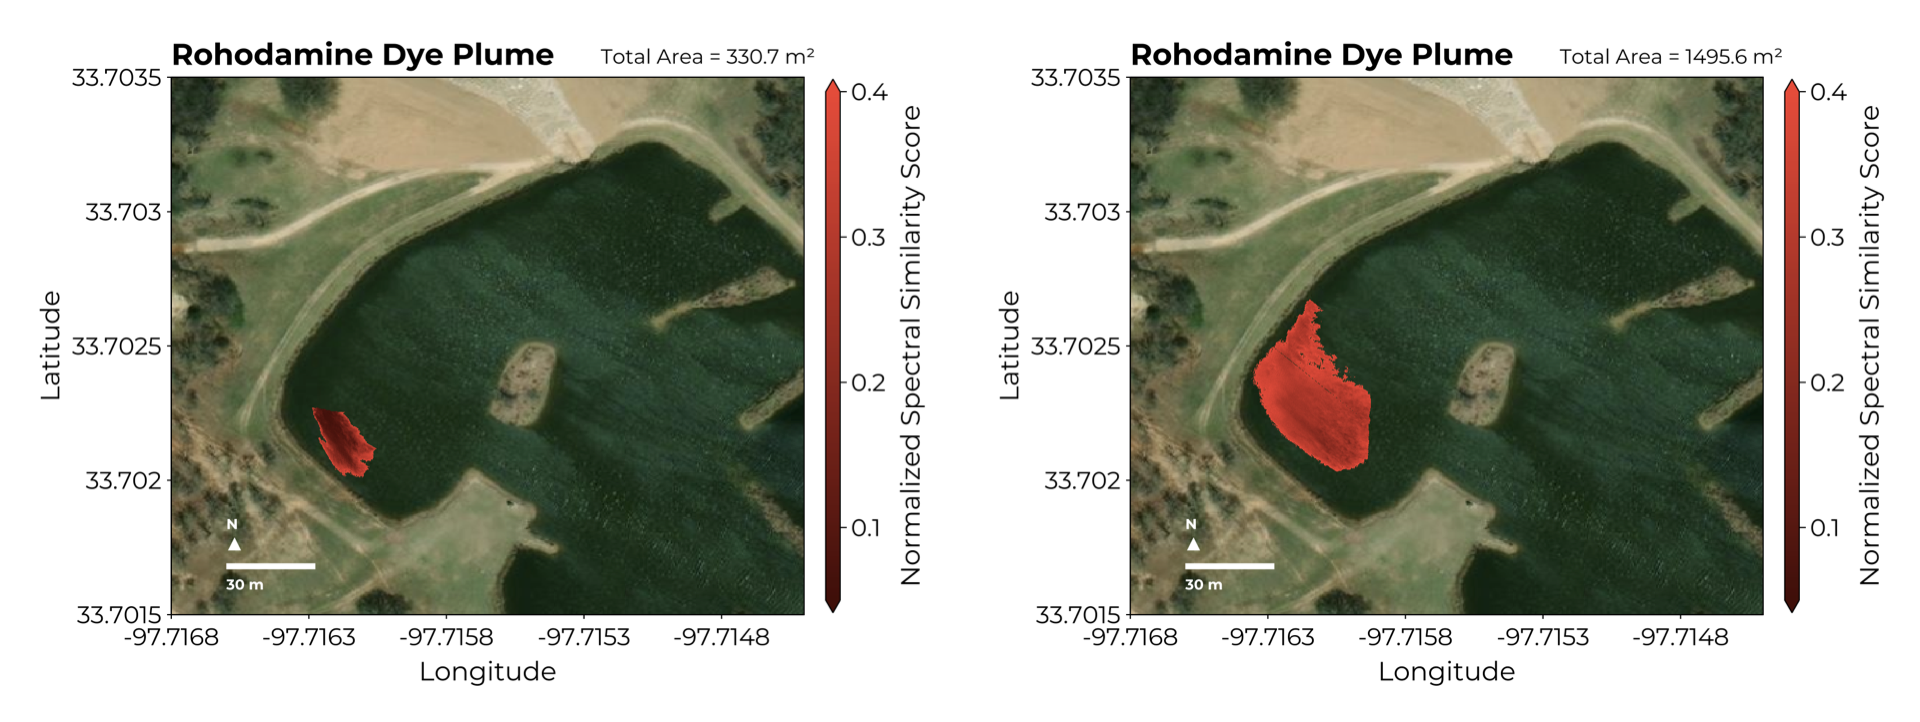
\includegraphics[width=17.0cm]{paper/figures/results/rhodamine.png}
\end{adjustwidth}
\caption{Using the spectral endmember assigned to Rhodamine from the trained GTM together with the NS3, we are able to map the evolution of the dye plume across two UAV flights. (\textbf{left}) The initial dye plume corresponding to a total area of $330.7$ $m^2$. (\textbf{right}) The same dye plume imaged approximately 15 minutes later now subsumes a total area of $1495.6$ $m^2$.\label{fig:rhodamine-map}}
\end{figure}  




%%%%%%%%%%%%%%%%%%%%%%%%%%%%%%%%%%%%%%%%%%
\section{Discussion}

- Use of UAV-based HSI for water quality assessment is becoming increasingly popular
- Most studies have focused on supervised techniques mapping captured spectra to specific parameters of interest 
- This approach relies on reference data which are expensive to collect and require prior knowledge of expected sources in order to select appropriate sensors 
- Spectral unmixing provides an HSI-only alternative however this approach relies on libraries of known endmember spectra
- Most studies exploring endmember extraction from UAV-based HSI are focused on extracting pure endmembers which can then be utilized by satellite based HSI

% smart collection of reference data
- The map of the distribution of GTM classes throughout the pond in Fig~\ref{fig:gtm-water} reveals the significant spatial variability typical of inland water bodies. Knowledge of this distribution is highly relevant for the collection of in situ reference data where taking samples as little as a meter apart could clearly lead to significant differences in measurements. 
- As a consequence, one useful application for the GTM is for intelligent reference data collection.
- The ability of any supervised model to infer water quality parameters from captured HSI relies on a sufficient volume of reference measurements which reflect the true distribution in the water
- In our previous work, we demonstrated how autonomous in situ data collection leads to significantly greater data volumes, which in turn, improves water parameter inversion models. 
- Using the distribution obtained by the GTM, an autonomous boat can be routed to maximially sample the observed distribution
- Cite papers where this has been done in other contexts... e.g. guided navigation of autonomous boat based on some cost function, for example, like the expected improvement functions used for Bayesian optimization strategies.
- Such a strategy would likely reduce the sampling time and improve data quality by sampling a broader portion of the distribution. 
- Since the GTM captures the distribution of observed spectra, we are also not constrained to the distribution of a single parameter as measured by the boat
- That is, we previously observed the distributions for parameters like CDOM, Chlorophyll, Temperature, Turbidity, Blue-green algae, etc. were highly dissimilar so that guiding the boat using a single reference sensor would not accurately reflect the comprehensive distribution of water composition.

\subsection{Summary of GTM applications in our paper}
\subsection{Comparison to other existing approaches in literature}
- Is there much done for classification in real time? 
\subsection{Comparison to Spectral Unmixing}
- Here we can re-interpret the GTM model as performing a type of Bayesian spectral unmixing and suggest how the method could be further extended to work in this domain. Critically, other traditional methods work by observing that pure endmembers form the vertices of a simplex. 

\subsection{Other applications of GTM}
- Discuss use of GTM means/modes/responsibilities feature transformer for supervised models (e.g. better than PCA) 
- Use of GTM classes to aid autonomous data collection by identification of "interesting" regons


- Drones can be equipped with HSI and compute to enable rapid generation of spectral indices like the NDVI for applications such as precision agriculture \cite{horstrand2019uav}

- Mention how Bishop suggests extensions to GTM for on-line learning which could be used to accelerate training for large HSI datasets


%%%%%%%%%%%%%%%%%%%%%%%%%%%%%%%%%%%%%%%%%%
\section{Conclusions}


%%%%%%%%%%%%%%%%%%%%%%%%%%%%%%%%%%%%%%%%%%
\vspace{6pt} 

%%%%%%%%%%%%%%%%%%%%%%%%%%%%%%%%%%%%%%%%%%
%% optional
%\supplementary{The following supporting information can be downloaded at:  \linksupplementary{s1}, Figure S1: title; Table S1: title; Video S1: title.}

% Only for journal Methods and Protocols:
% If you wish to submit a video article, please do so with any other supplementary material.
% \supplementary{The following supporting information can be downloaded at: \linksupplementary{s1}, Figure S1: title; Table S1: title; Video S1: title. A supporting video article is available at doi: link.}

% Only for journal Hardware:
% If you wish to submit a video article, please do so with any other supplementary material.
% \supplementary{The following supporting information can be downloaded at: \linksupplementary{s1}, Figure S1: title; Table S1: title; Video S1: title.\vspace{6pt}\\
%\begin{tabularx}{\textwidth}{lll}
%\toprule
%\textbf{Name} & \textbf{Type} & \textbf{Description} \\
%\midrule
%S1 & Python script (.py) & Script of python source code used in XX \\
%S2 & Text (.txt) & Script of modelling code used to make Figure X \\
%S3 & Text (.txt) & Raw data from experiment X \\
%S4 & Video (.mp4) & Video demonstrating the hardware in use \\
%... & ... & ... \\
%\bottomrule
%\end{tabularx}
%}

%%%%%%%%%%%%%%%%%%%%%%%%%%%%%%%%%%%%%%%%%%
\authorcontributions{FIXME}

\funding{FIXME}

\institutionalreview{Not applicable}

\informedconsent{Not applicable}

\dataavailability{We encourage all authors of articles published in MDPI journals to share their research data. In this section, please provide details regarding where data supporting reported results can be found, including links to publicly archived datasets analyzed or generated during the study. Where no new data were created, or where data is unavailable due to privacy or ethical restrictions, a statement is still required. Suggested Data Availability Statements are available in section ``MDPI Research Data Policies'' at \url{https://www.mdpi.com/ethics}.} 


\acknowledgments{In this section you can acknowledge any support given which is not covered by the author contribution or funding sections. This may include administrative and technical support, or donations in kind (e.g., materials used for experiments).}

\conflictsofinterest{Declare conflicts of interest or state ``The authors declare no conflicts of interest.'' Authors must identify and declare any personal circumstances or interest that may be perceived as inappropriately influencing the representation or interpretation of reported research results. Any role of the funders in the design of the study; in the collection, analyses or interpretation of data; in the writing of the manuscript; or in the decision to publish the results must be declared in this section. If there is no role, please state ``The funders had no role in the design of the study; in the collection, analyses, or interpretation of data; in the writing of the manuscript; or in the decision to publish the results''.} 

%%%%%%%%%%%%%%%%%%%%%%%%%%%%%%%%%%%%%%%%%%
%% Optional

%% Only for journal Encyclopedia
%\entrylink{The Link to this entry published on the encyclopedia platform.}

\abbreviations{Abbreviations}{
The following abbreviations are used in this manuscript:\\

\noindent 
\begin{tabular}{@{}ll}
UAV & Unmanned Aerial Vehicle \\
GTM & Generative Topographic Mapping  \\
SOM & Self Organizing Map \\ 
HSI & Hyperspectral Image \\ 
PCA & Principal Component Analysis \\ 
tSNE & t-Distributed Stochastic Neighbor Embedding \\
MLJ & Machine Learning in Julia \\ 
VNIR & Visible + Near-Infrared \\
NDWI & Normalized Difference Water Index \\ 
NS3 & Normalized Spectral Similarity Score
\end{tabular}
}

%%%%%%%%%%%%%%%%%%%%%%%%%%%%%%%%%%%%%%%%%%
%% Optional
\appendixtitles{yes} % Leave argument "no" if all appendix headings stay EMPTY (then no dot is printed after "Appendix A"). If the appendix sections contain a heading then change the argument to "yes".
\appendixstart
\appendix
\section[\appendixname~\thesection]{Hyperparameter Search Results}

\begin{table}[H]
  \caption{The top 25 models from the hyperparameter search. A variety of GTM were trained to explore the the impact of varying m, $\alpha$, and s. The Bayesian Information Criterion (BIC) and Akaike Information Criterion (AIC) are given in the final two columns which can be used for hyperparameter selection. \label{tab:hp-search}}
  \begin{adjustwidth}{-\extralength}{0cm}
  \newcolumntype{C}{>{\centering\arraybackslash}X}
  \begin{tabularx}{\fulllength}{CCCCCC}
    \toprule
    \textbf{m} & \textbf{$\alpha$} & \textbf{s} & \textbf{k} & \textbf{BIC} & \textbf{AIC} \\
    \midrule
    \textbf{14} & \textbf{0.1} & \textbf{1.0} & \textbf{32} & \textbf{-1.918e8} & \textbf{-1.926e8}\\
    13 & 0.01 & 1.0 & 32 & -1.917e8 & -1.923e8\\
    16 & 0.01 & 1.5 & 32 & -1.917e8 & -1.926e8\\
    14 & 10.0 & 1.0 & 32 & -1.917e8 & -1.924e8\\
    16 & 0.001 & 1.5 & 32 & -1.917e8 & -1.926e8\\
    13 & 1.0 & 1.0 & 32 & -1.917e8 & -1.923e8\\
    13 & 10.0 & 1.0 & 32 & -1.917e8 & -1.923e8\\
    14 & 0.001 & 1.5 & 32 & -1.916e8 & -1.924e8\\
    13 & 0.1 & 1.0 & 32 & -1.916e8 & -1.923e8\\
    14 & 0.01 & 1.0 & 32 & -1.916e8 & -1.924e8\\
    15 & 0.01 & 1.5 & 32 & -1.916e8 & -1.925e8\\
    14 & 0.01 & 1.5 & 32 & -1.916e8 & -1.923e8\\
    15 & 1.0 & 1.0 & 32 & -1.916e8 & -1.924e8\\
    18 & 0.01 & 1.5 & 32 & -1.916e8 & -1.928e8\\
    12 & 0.01 & 1.0 & 32 & -1.916e8 & -1.921e8\\
    15 & 0.01 & 0.5 & 32 & -1.915e8 & -1.924e8\\
    17 & 1.0 & 1.0 & 32 & -1.915e8 & -1.926e8\\
    16 & 0.1 & 1.0 & 32 & -1.915e8 & -1.925e8\\
    18 & 0.001 & 1.5 & 32 & -1.915e8 & -1.928e8\\
    13 & 0.001 & 1.0 & 32 & -1.915e8 & -1.922e8\\
    12 & 1.0 & 1.0 & 32 & -1.915e8 & -1.921e8\\
    17 & 0.001 & 1.5 & 32 & -1.915e8 & -1.926e8\\
    15 & 0.001 & 1.5 & 32 & -1.915e8 & -1.923e8\\
    15 & 10.0 & 1.0 & 32 & -1.915e8 & -1.923e8\\
    12 & 0.1 & 1.5 & 32 & -1.915e8 & -1.92e8\\
    \bottomrule
  \end{tabularx}
  \end{adjustwidth}
\end{table}


%%%%%%%%%%%%%%%%%%%%%%%%%%%%%%%%%%%%%%%%%%
\begin{adjustwidth}{-\extralength}{0cm}
%\printendnotes[custom] % Un-comment to print a list of endnotes

\reftitle{References}

%=====================================
% References, variant A: external bibliography
%=====================================
\bibliography{paper/references.bib}

%%%%%%%%%%%%%%%%%%%%%%%%%%%%%%%%%%%%%%%%%%
\PublishersNote{}
\end{adjustwidth}
\end{document}

